\section{统一目标与更新场的数值核验}
\label{evidence:reconstruction}

本节对应实验目录 \path{results/book-reconstruction/}。原始参数、随机种子、词表规模、误差定义、代码版本与各项数值判据保存在 \path{results/book-reconstruction/metadata.json}；图中的量从同一组可枚举 categorical 分布计算。该实验核对数学恒等式、局部曲率、更新场是否具有势函数及方差控制，证据范围为固定 prefix 的完整动作枚举。

本轮实验枚举 $360$ 组配置，恒等式与导数核验的最大绝对残差为 $4.44\times10^{-15}$。实验分别报告 Part--BPO 与 Mean--BPO 的均方分解、四目标的归一化商坐标关系、anchor 处的梯度与 Hessian、MDPO 的 KL gap，以及粗粒化 BPO 的交叉偏导。每项计算采用对应定理规定的固定 anchor 和支持集；PyTorch 自动微分所得 Jacobian 与独立解析式对照。更新场的非零 curl 核验使用定理~\ref{opd:field-curl} 的三 token 反例。

这些数值核验与此前四 token 的 400 步优化实验互补。前者检查数学关系及其实现；后者比较给定初始化、学习率、优化器和预算下到达自身总体解的距离。Qwen 固定 prefix KL 表检验估计器误差，Pythia baseline 表保留历史记录，hard-sync 实验检验受控分布动力学；各项不能替代完整 GSM8K 训练效果。

为单独检查初始梯度尺度，新增实验从 $q=(0.5,0.3,0.2)$ 出发，固定 $t=(0.2,0.3,0.5)$ 与 $\eta=0.8$。Part、Mean 与 $\eta L_{\mathrm{BPO}}$ 全部使用普通 logit 梯度下降，步长 $0.4$，运行 $1000$ 步。三者在初值具有相同梯度。最终 Part 与 BPO 到 Gibbs 的 TV 分别为 $3.05\times10^{-16}$ 与 $2.22\times10^{-16}$；Mean 的梯度范数为 $2.06\times10^{-16}$，到 Gibbs 的 TV 仍为 $0.0370627$。这个差异来自总体目标，有限 inner 轨迹保存于 \path{results/book-reconstruction/finite-inner.csv}。

受限学生族实验取 $q=(1/3,1/3,1/3)$、$t=(0.1,0.7,0.2)$、$\eta=1$，学生 logits 为 $(z,0,0)$。BPO 的解析最小点 $z=-1.3195286648$ 处，Part 导数为 $0.03543884357$。它补充了前一组实验：完整可表示时共同 Gibbs target 可以恢复，表达受限时连总体最优投影也会不同。

\begin{figure}[ht]
\centering
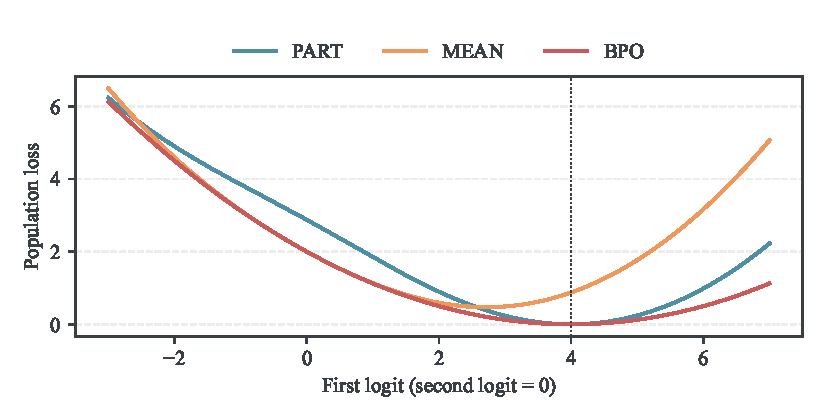
\includegraphics[width=0.96\textwidth]{../../results/book-reconstruction/identities.pdf}
\caption{二元 categorical 分布下三种同尺度回归目标。$q=(1/2,1/2)$、$f=(2,-2)$、$\eta=1$，第二个 logit 固定为零；虚线 $z_1=4$ 对应共同 Gibbs target。Part 与 BPO 的总体零损失位置相同，Mean 的最优点不同。}
\label{evidence:identities-figure}
\end{figure}
